\section{Variations over an algorithm}
\subsection{}

\begin{frame}
\frametitleTC{Foreword}
\framesubtitleTC{}
\myPause
 \begin{itemize}[<+-| alert@+>]
 \item Now we know enough for our purposes about the PID control law.
 \item We also know that to turn the LTI law into an algorithm, there are some nonlinear additions
       to care about (e.g., antiwindup).
 \item Such additions are not just ``implementation choices''; they do not fit into the LTI
       context, but nonetheless \TC{need addressing systematically}.
 \item Otherwise the (wrong) conclusion is easily reached that ``the theory is neat but too
       simplistic to be useful in the real world''...
 \item ...and controls soon become an inextricable and unmaintainable\\
       \emph{spaghetti} code, where -- inexplicably from the control scientist's\\
       viewpoint --  problems are tackled by adding further complexity\\
       (apologies for not resisting the temptation to this remark).
 \end{itemize}
\end{frame}

\begin{frame}
\frametitleTC{Foreword}
\framesubtitleTC{}
\myPause
 \begin{itemize}[<+-| alert@+>]
 \item Anticipating a bit, we want to reach the following conclusions:
       \begin{itemize}[<+-| alert@+>]
       \item you tune and assess a PID, or more in general a control scheme,\\
             in the LTI context,
       \item and then you take care of ``nonlinear additions'' in such a way\\
             to not contradict/disrupt your LTI findings;
       \item but to make this possible, a PID block must contain something\\
             more than the LTI law (and this we are going to study a bit).
       \end{itemize}
 \item Given the available space, here we address ``algorithm variations'' -- i.e.,\\
       the ``something more'' above -- as for three aspects only:
       \begin{itemize}[<+-| alert@+>]
       \item positional versus incremental form,
       \item how antiwindup is realised,
       \item and (a few examples of) what can be added to ease interconnecting\\
             a PID with other controllers in the same overall system.
       \end{itemize}
 \item \vfill Once again, much more in advanced control (technology) courses.
 \end{itemize}
\end{frame}

\begin{frame}
\frametitleTC{Positional vs. incremental realisation}
\framesubtitleTC{Definition}
\myPause
 \begin{itemize}[<+-| alert@+>]
 \item For simplicity in this treatise we refer to a PI, conceptually nothing changes\\
       if D is added.
 \item \vspace{2mm} \TC{Positional} realisation:\\
       $e(k)$ is used to compute $u(k)$.
 \item \vspace{2mm} \TC{Incremental} realisation:\\
       first the variation of $u(k)$ wrt its previous value is computed,\\
       and then this variation is added to the previous value of $u$ to get\\
       the current one.
 \end{itemize}
\end{frame}

\begin{frame}
\frametitleTC{Positional vs. incremental realisation}
\framesubtitleTC{The variation operator}
\myPause
 \begin{itemize}[<+-| alert@+>]
 \item We define the \TC{variation operator} $\Delta$ with reference to the one-step advance\\
       one $z$, as
       \begin{displaymath}
        \Delta := 1-z^{-1}.
       \end{displaymath}
 \item As a consequence, since in the time domain the variation of a signal $v(k)$
       is naturally defined as
       \begin{displaymath}
        \Delta v(k) = v(k)-v(k-1),
       \end{displaymath}
       we can give the formal multiplication by $\Delta$ an operatorial sense,\\
       exactly as we in fact already did for the formal multiplication by $z$. 
 \end{itemize}
\end{frame}


\begin{frame}
\frametitleTC{Positional vs. incremental realisation}
\framesubtitleTC{An incremental PI}
\myPause
 \begin{itemize}[<+-| alert@+>]
 \item The positional PI law, as we already know, is
       \begin{displaymath}
        \begin{array}{rcl}
         u_P(k) &=& K e(k) \\
         u_I(k) &=& u_I(k-1) + \cfrac{KT_s}{T_i} e(k)
        \end{array}
       \end{displaymath}
 \item hence the incremental one readily stems from the definition of $\Delta$, as
       \begin{displaymath}
        \begin{array}{rcl}
         \Delta u_P(k) &=& K \Delta e(k) \\
         \Delta u_I(k) &=& \cfrac{KT_s}{T_i} e(k)
        \end{array}
       \end{displaymath}
       and obviously the control variation $\Delta u(k)$ is just $\Delta u_P(k)+\Delta u_I(k)$.
 \end{itemize}
\end{frame}

\begin{frame}
\frametitleTC{Incremental realisation}
\framesubtitleTC{Pros and cons}
\myPause
 \begin{itemize}[<+-| alert@+>]
 \item Pros:
       \begin{itemize}[<+-| alert@+>]
       \item can use all the available precision for the control \TC{variation},\\
             i.e., just one many-bits register is needed to store $u(k)$, which may be\\
             relevant e.g. when constrained to integer-numbers arithmetic like in the\\
             Linux kernel;
       \item easy to realise antiwindup and tracking (see algorithm later on);
       \end{itemize}
 \item Cons:
       \begin{itemize}[<+-| alert@+>]
       \item for the same reason above, unnatural to realise antiwindup if not in the\\
             ``natural way'' mentioned above (no pun intended);
       \item in the absence of I action \TC{MUST} be in automatic mode when the\\
             set point is varied, otherwise that variation is lost forever.
       \end{itemize}
 \end{itemize}
\end{frame}

\begin{frame}[fragile]
\frametitleTC{Positional vs. incremental realisation}
\framesubtitleTC{PI algorithm example -- positional version from slide~\ref{pag:PI-complete-alg}}
\myPause
 \begin{itemize}[<+-| alert@+>]
 \item[]{\scriptsize
   \begin{verbatim}
// POSITIONAL                                // INCREMENTAL
e      = w-y;                                e       = w-y; 
up     = K*e;                                Delta_e = e-e_old;              
if not TS then                               if not TS then    
   ui  = ui_old+K*Ts/Ti*e;                      Delta_up = K*Delta_e;
   u   = up+ui;                                 Delta_ui = K*Ts/Ti*e;
                                                u        = u_old+Delta_up+Delta_ui;
else                                         else                 
   u   = TR;                                    u        = TR;
end if;                                      end if
u      = max(umin,min(umax,u));              u     = max(umin,min(umax,u));
ui_old = u-up;                               u_old = u;
                                             e_old = e;
   \end{verbatim}
   }
 \item Exercise: try this in Modelica.
 \end{itemize}
\end{frame}

\begin{frame}[fragile]
\frametitleTC{Antiwindup methods}
\framesubtitleTC{}
\myPause
 \begin{itemize}[<+-| alert@+>]
 \item Till now we have been realising antiwindup
       \begin{itemize}[<+-| alert@+>]
       \item either by \TC{integral recomputation} in the positional form, i.e.,\\
             \verb£ u      = max(umin,min(umax,u));£\\
             \verb£ ui_old = u-up;                 £
       \item or by just computing $\Delta u$ (incremental form) and clamping the state of\\
             the \TC{output integrator} that sums the subsequent variations into $u$. 
       \end{itemize}
  \item \vspace{2mm} These methods came naturally, but there are alternatives, and these\\
        may impact the control loop behaviour in the face of large input\\
        (set point or disturbance) swings.
  \item We just see one example, namely antiwindup by \TC{internal positive\\
        feedback}. % NOTE in the future may add actuation error feedback, possibly with actuator model
  \end{itemize}
\end{frame}

\begin{frame}
\frametitleTC{Antiwindup methods}
\framesubtitleTC{PI with antiwindup by internal positive feedback}
\myPause
 \begin{itemize}[<+-| alert@+>]
  \item Block diagram
        \begin{center}
         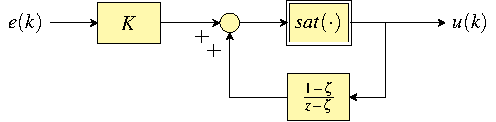
\includegraphics[width=0.60\columnwidth]{./Unit-07/img/PI-AW-intFB.pdf}
        \end{center}
        where for compactness we use the pure DT parametrisation $(K,\zeta)$.
  \item The saturation function is defined as
        \begin{displaymath}
         sat(x) = \begin{cases}
                   \; x_{min} & \quad x < x_{min} \\
                   \; x       & \quad x_{min} \leq x \leq x_{max} \\
                   \; x_{max} & \quad x > x_{max}
                  \end{cases}
        \end{displaymath}
  \end{itemize}
\end{frame}

\begin{frame}
\frametitleTC{Antiwindup by internal positive feedback}
\framesubtitleTC{Operation}
\myPause
 \begin{center}
  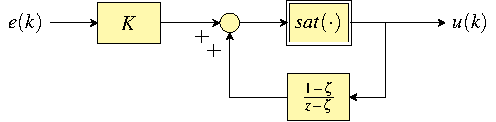
\includegraphics[width=0.45\columnwidth]{./Unit-07/img/PI-AW-intFB.pdf}
 \end{center}
 \myPause
 \begin{itemize}[<+-| alert@+>]
  \item In the absence of saturation the $sat(\cdot)$ block has output=input, hence in transfer function form
        (mind the \red{positive} feedback) we get
        \begin{displaymath}
         \frac{u(k)}{e(k)} = K \frac{1}{1\mathbf{\red{-}}\frac{1-\zeta}{z-\zeta}}
                           = K \frac{z-\zeta}{z-\cancel{\zeta}-1+\cancel{\zeta}}
                           = K \frac{z-\zeta}{z-1}
        \end{displaymath}
        which is a PI as desired.
  \item In the presence of saturation the loop inside the PI opens and the\\
        integrator (see above) ceases to exist  $\Rightarrow$ no windup.
  \end{itemize}
\end{frame}

\begin{frame}
\frametitleTC{Antiwindup PI}
\framesubtitleTC{Modelica (block diagram) representation -- positional realisation}
\myPause
 \begin{center}
  %rsvg-convert -f pdf -o PI_nnn.pdf PI_nnn.svg
  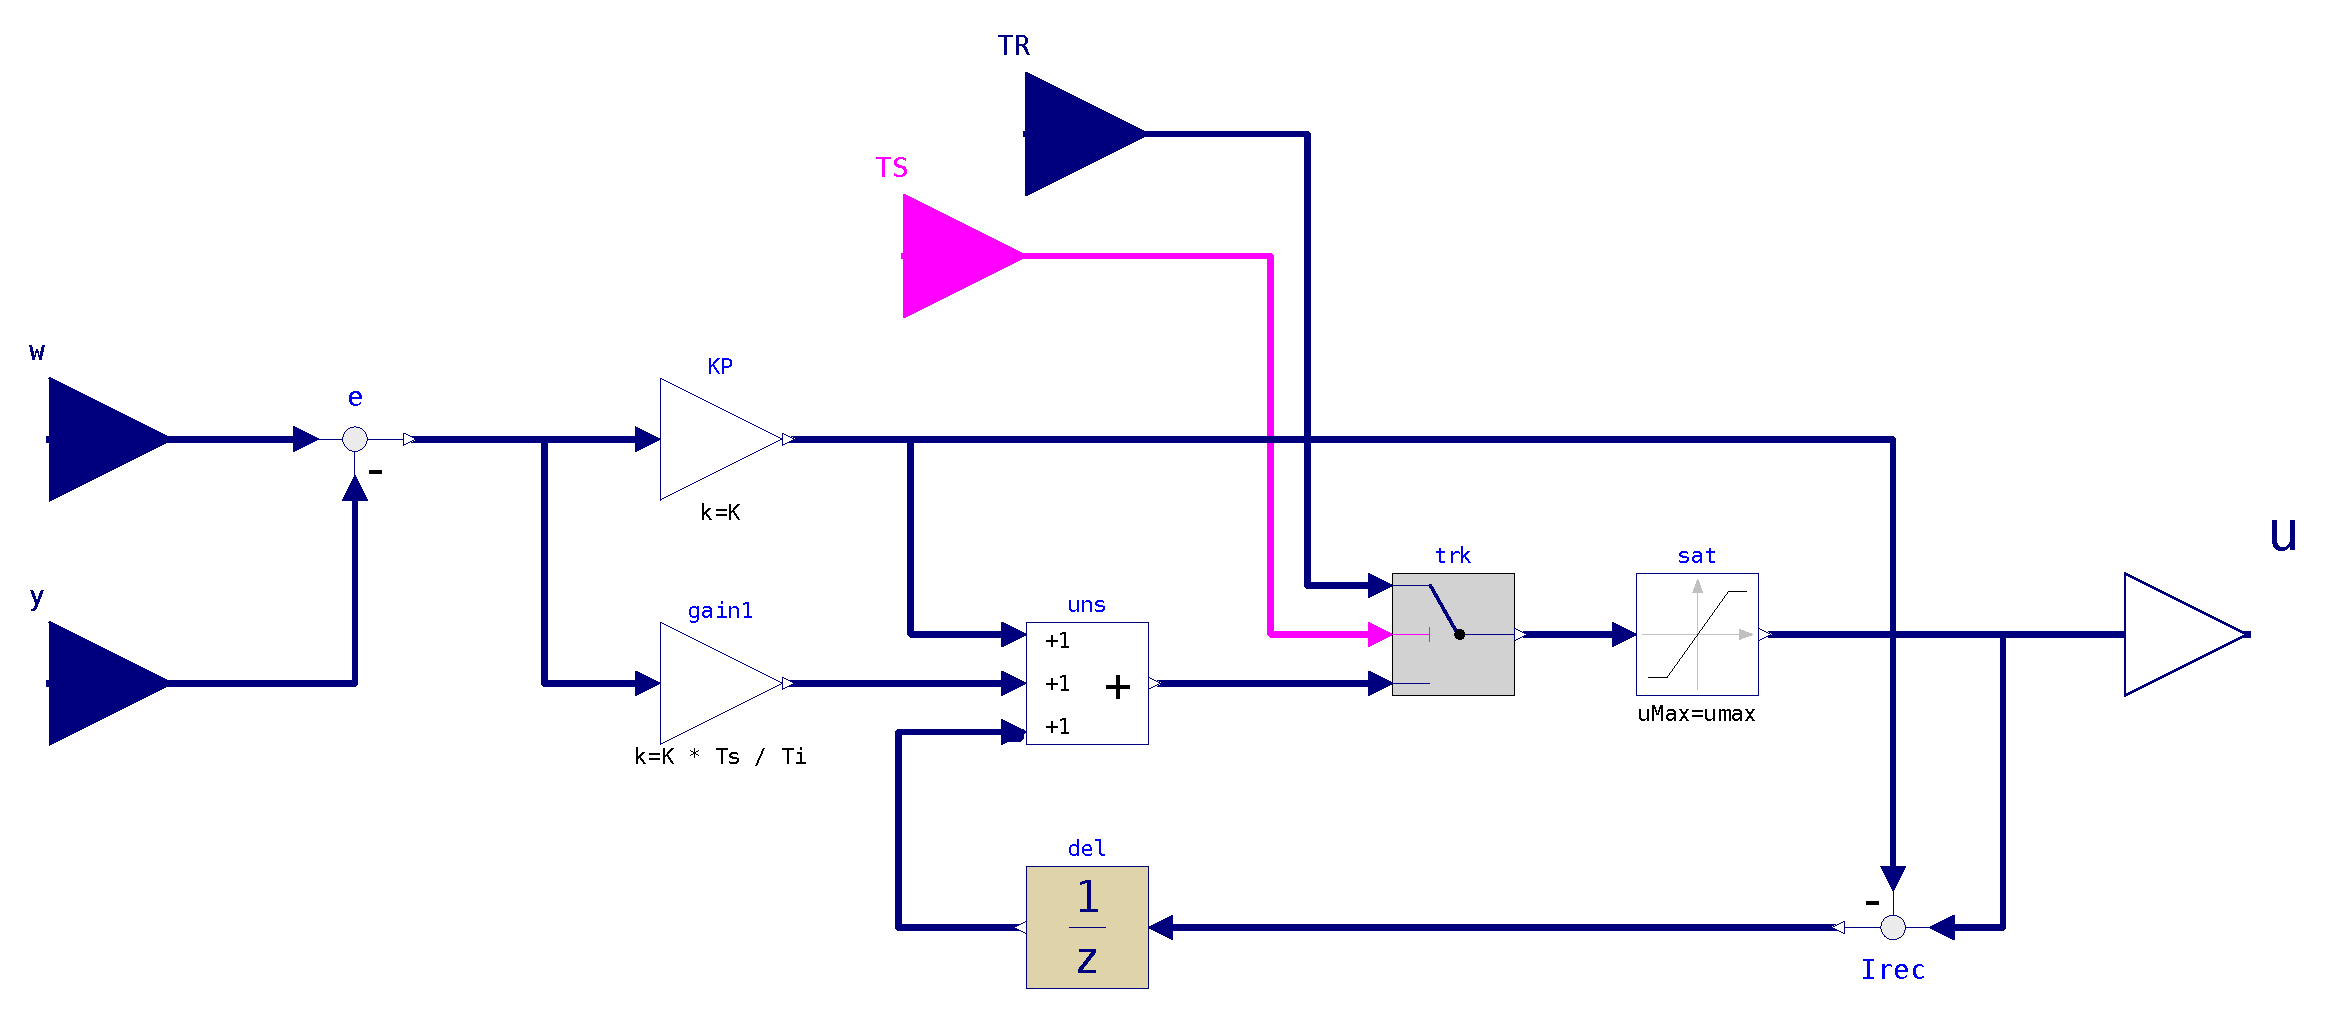
\includegraphics[width=0.80\columnwidth]{./Unit-07/img/PI_POS.pdf}\\
 \end{center}
\end{frame}

\begin{frame}
\frametitleTC{Antiwindup PI}
\framesubtitleTC{Modelica (block diagram) representation -- incremental realisation}
\myPause
 \begin{center}
  %rsvg-convert -f pdf -o PI_nnn.pdf PI_nnn.svg
  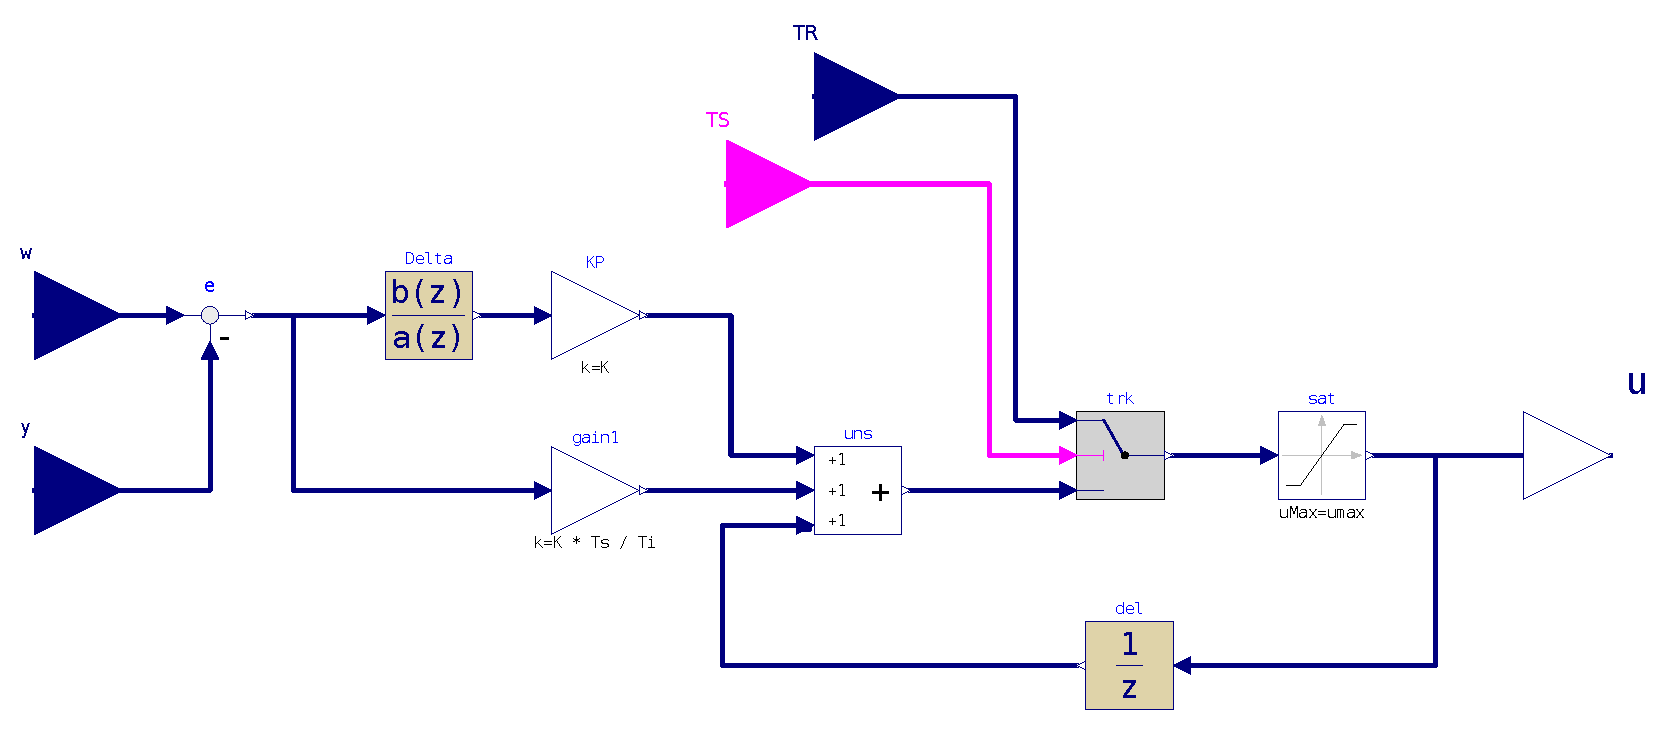
\includegraphics[width=0.80\columnwidth]{./Unit-07/img/PI_INC.pdf}\\
 \end{center}
\end{frame}

\begin{frame}
\frametitleTC{Antiwindup PI}
\framesubtitleTC{Modelica (block diagram) representation -- internal feedback realisation}
\myPause
 \begin{center}
  %rsvg-convert -f pdf -o PI_nnn.pdf PI_nnn.svg
  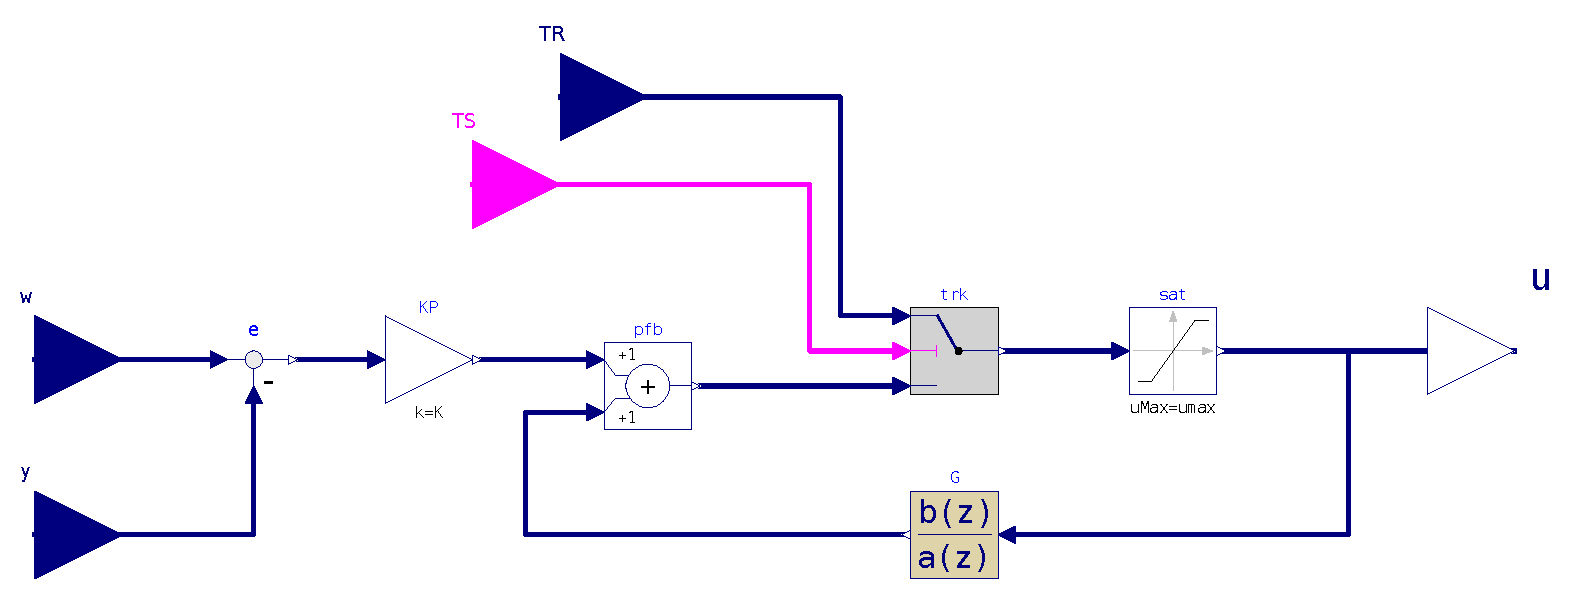
\includegraphics[width=0.80\columnwidth]{./Unit-07/img/PI_IFB.pdf}\\
 \end{center}
\end{frame}

\begin{frame}
\frametitleTC{Antiwindup PI}
\framesubtitleTC{Results and comparison -- set point step large enough to provoke control saturation}
\myPause
 \begin{columns}
  \column[T]{0.70\textwidth}
   \begin{tabular}{ll}
    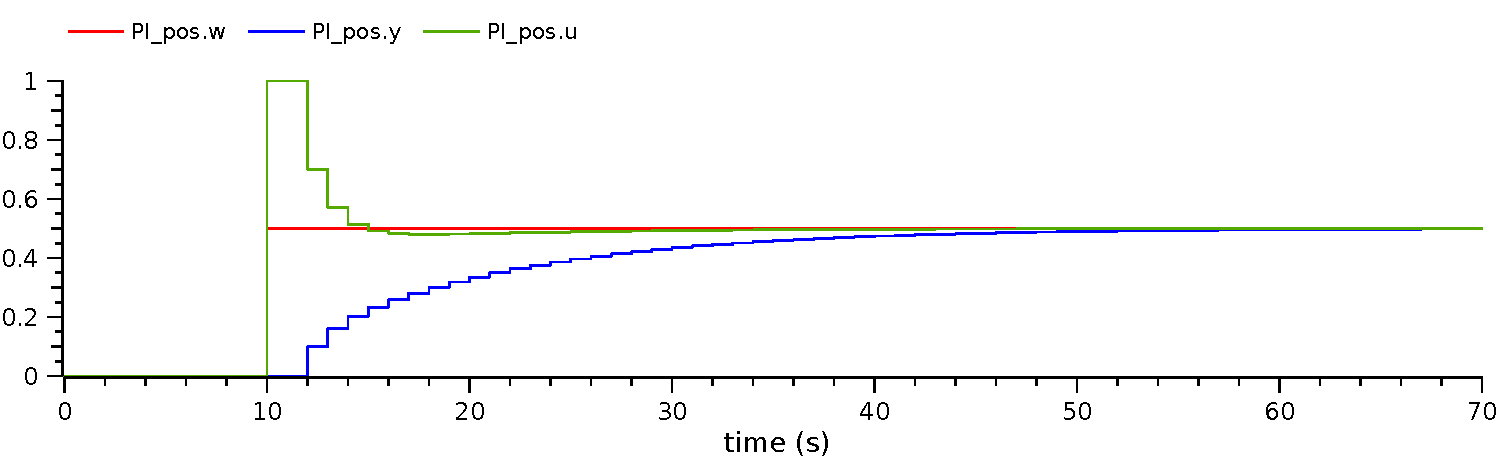
\includegraphics[width=0.70\columnwidth]{./Unit-07/img/PI_POS-wyu.pdf} & Positional
   \end{tabular}
   \begin{tabular}{ll}
    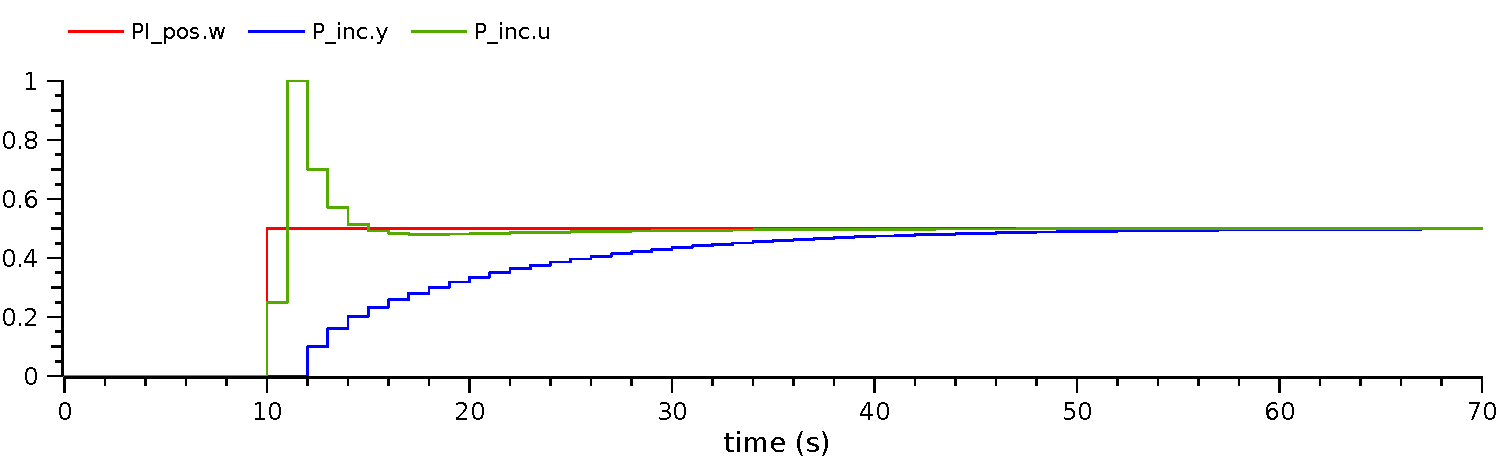
\includegraphics[width=0.70\columnwidth]{./Unit-07/img/PI_INC-wyu.pdf} & Incremental\\
   \end{tabular}
   \begin{tabular}{ll}
    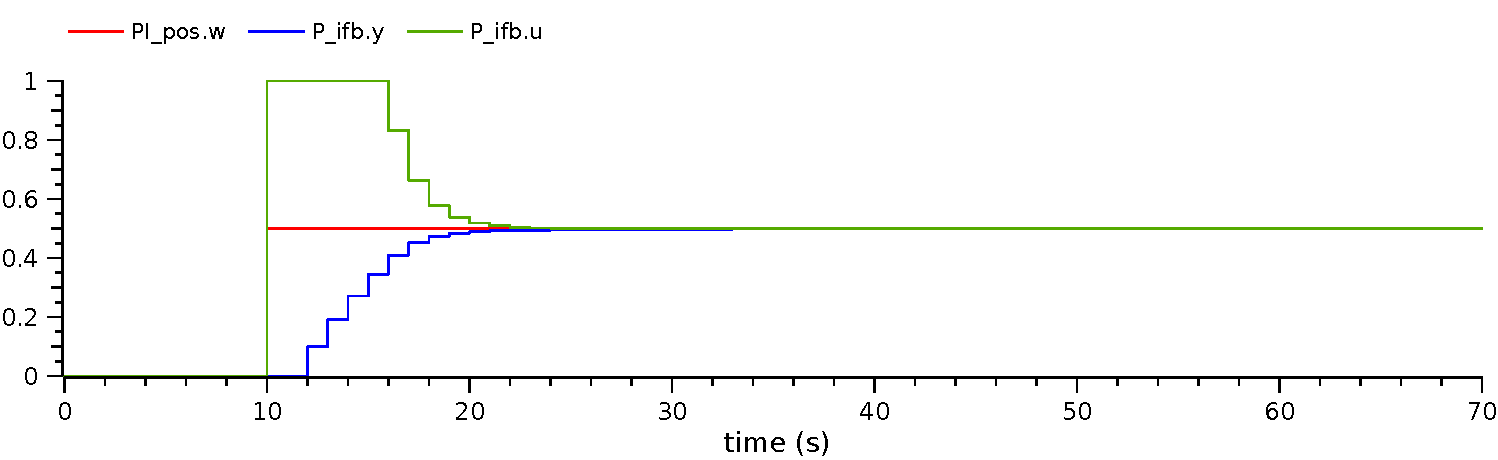
\includegraphics[width=0.70\columnwidth]{./Unit-07/img/PI_IFB-wyu.pdf} & Int. feedback\\
   \end{tabular}
  \column[T]{0.30\textwidth}
   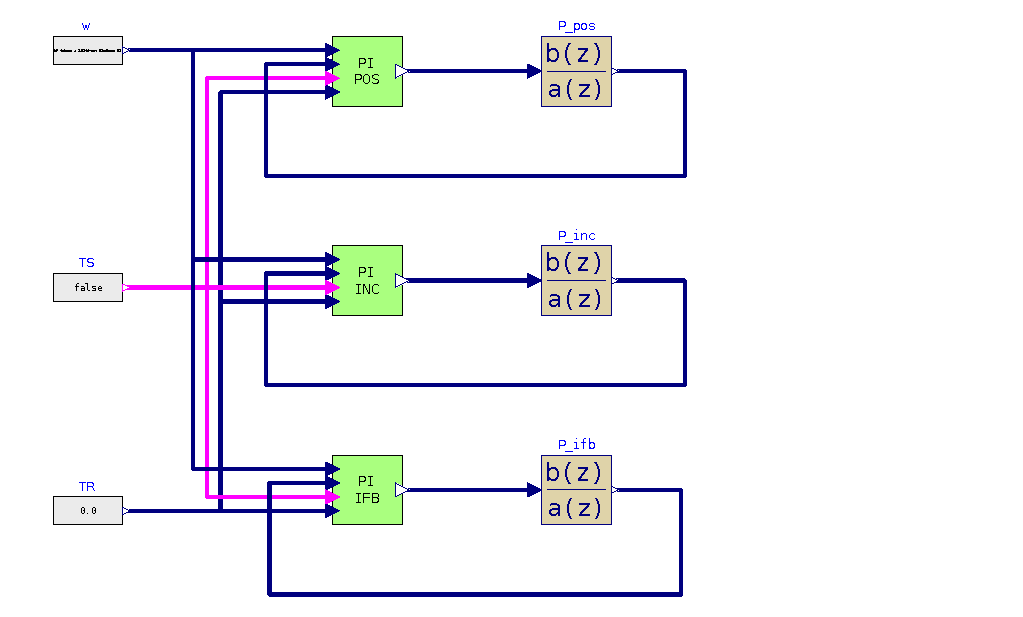
\includegraphics[width=1.20\columnwidth]{./Unit-07/img/AWtypes_ex01.pdf}\\
 \end{columns}
\end{frame}

